\documentclass[border=12pt]{standalone}
\usepackage{amssymb}
\usepackage{tikz}
\usetikzlibrary{arrows.meta, decorations.pathreplacing, calc, bending, positioning, shapes.geometric}

% Project palette
\definecolor{cnavy}{HTML}{0E2747}
\definecolor{corange}{HTML}{E8573F}
\definecolor{cgreen}{HTML}{3B9B6D}
\definecolor{cslate}{HTML}{5B6680}
\definecolor{cmuted}{HTML}{9B9484}
\definecolor{ccream}{HTML}{FAFAF6}
\definecolor{cheart}{HTML}{C73633}
\definecolor{cspade}{HTML}{1A1A1A}

\begin{document}
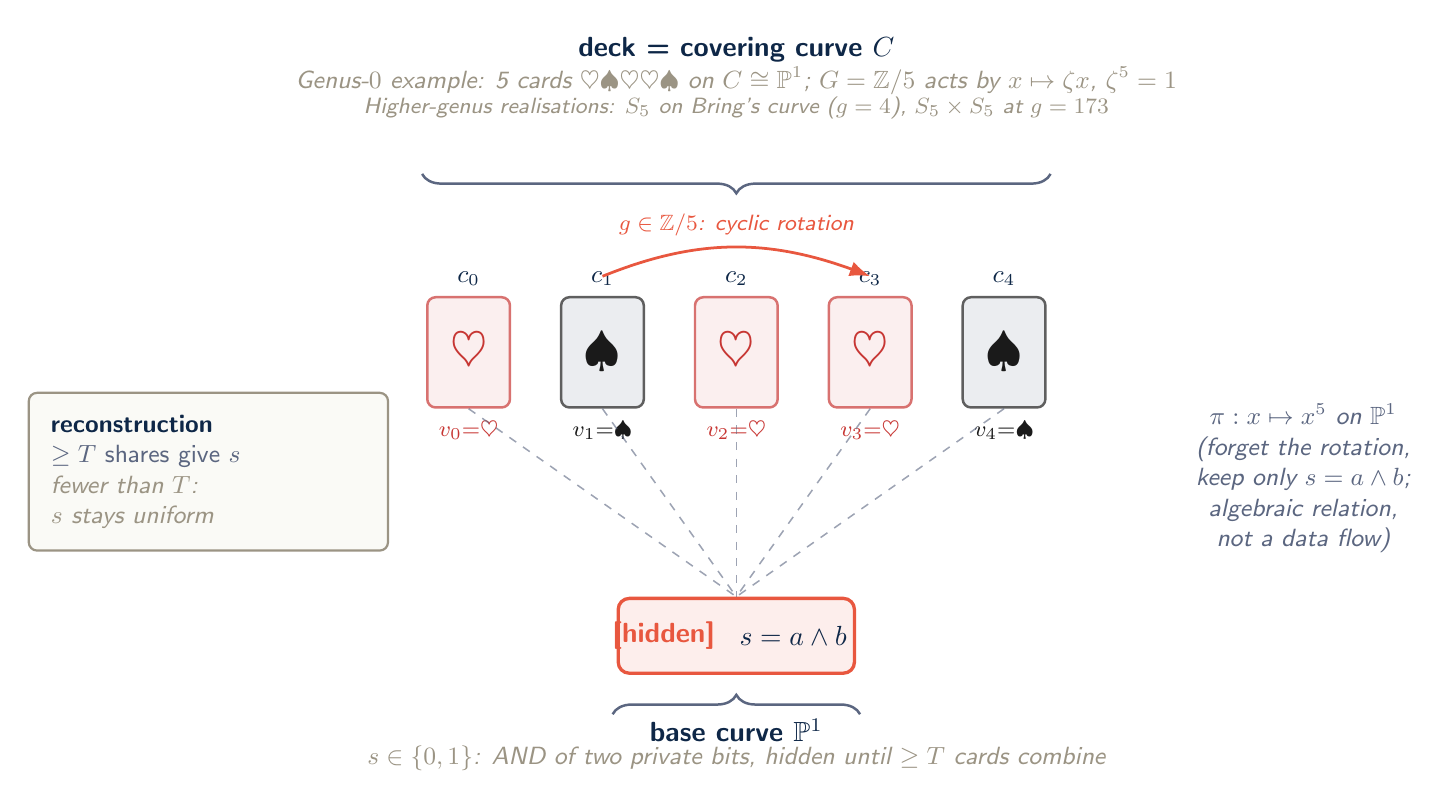
\begin{tikzpicture}[
  cardH/.style={
    rectangle, rounded corners=3pt, draw=cheart!70, fill=cheart!8,
    line width=0.9pt, minimum width=1.05cm, minimum height=1.4cm, inner sep=0pt
  },
  cardS/.style={
    rectangle, rounded corners=3pt, draw=cspade!70, fill=cslate!12,
    line width=0.9pt, minimum width=1.05cm, minimum height=1.4cm, inner sep=0pt
  },
  secretbox/.style={
    rectangle, rounded corners=4pt, draw=corange, fill=corange!10,
    line width=1.2pt, minimum width=3.0cm, minimum height=0.95cm, inner sep=3pt
  },
  marrow/.style={dashed, draw=cslate, line width=0.55pt, opacity=0.6},
  gcurve/.style={-{Latex[length=2.6mm]}, draw=corange, line width=1.0pt},
  cbrace/.style={decorate, decoration={brace, amplitude=7pt}, line width=0.9pt, draw=cslate},
  font=\sffamily
]

% ============================================================
% Five cards with concrete suits (den Boer 1989 style 5-card example):
% pattern ♥ ♠ ♥ ♥ ♠ on positions c_0..c_4.
\node[cardH] (c0) at (0*1.7, 3.1) {};
\node[cardS] (c1) at (1*1.7, 3.1) {};
\node[cardH] (c2) at (2*1.7, 3.1) {};
\node[cardH] (c3) at (3*1.7, 3.1) {};
\node[cardS] (c4) at (4*1.7, 3.1) {};

% Card index labels (small, above each card)
\foreach \i in {0,...,4} {
  \node[cnavy, font=\sffamily\bfseries\small] at ($(c\i.north)+(0,0.22)$) {$c_{\i}$};
}

% Suit symbols centered in each card
\node[cheart, font=\LARGE] at (c0.center) {$\heartsuit$};
\node[cspade, font=\LARGE] at (c1.center) {$\spadesuit$};
\node[cheart, font=\LARGE] at (c2.center) {$\heartsuit$};
\node[cheart, font=\LARGE] at (c3.center) {$\heartsuit$};
\node[cspade, font=\LARGE] at (c4.center) {$\spadesuit$};

% Share-value labels below cards (v_i = suit shown by the card)
\node[cheart, font=\sffamily\bfseries\footnotesize] at ($(c0.south)+(0,-0.28)$) {$v_0{=}\heartsuit$};
\node[cspade, font=\sffamily\bfseries\footnotesize] at ($(c1.south)+(0,-0.28)$) {$v_1{=}\spadesuit$};
\node[cheart, font=\sffamily\bfseries\footnotesize] at ($(c2.south)+(0,-0.28)$) {$v_2{=}\heartsuit$};
\node[cheart, font=\sffamily\bfseries\footnotesize] at ($(c3.south)+(0,-0.28)$) {$v_3{=}\heartsuit$};
\node[cspade, font=\sffamily\bfseries\footnotesize] at ($(c4.south)+(0,-0.28)$) {$v_4{=}\spadesuit$};

% Curved monodromy arrow: cyclic rotation g ∈ Z/5 permutes cards
\draw[gcurve, bend left=22] ($(c1.north)+(0,0.25)$) to
  node[midway, above=0pt, font=\sffamily\itshape\footnotesize, color=corange] {$g \in \mathbb{Z}/5$: cyclic rotation}
  ($(c3.north)+(0,0.25)$);

% Brace + labels above the deck (subtitles lifted clear of the brace)
\draw[cbrace] ($(c4.north east)+(0.05,1.55)$) -- ($(c0.north west)+(-0.05,1.55)$);
\node[cnavy,  font=\sffamily\bfseries] at (3.4, 6.95) {deck = covering curve $C$};
\node[cmuted, font=\sffamily\itshape\small] at (3.4, 6.55)
  {Genus-$0$ example: 5 cards $\heartsuit\spadesuit\heartsuit\heartsuit\spadesuit$ on $C \cong \mathbb{P}^{1}$; $G = \mathbb{Z}/5$ acts by $x \mapsto \zeta x$, $\zeta^{5}=1$};
\node[cmuted, font=\sffamily\itshape\footnotesize] at (3.4, 6.20)
  {Higher-genus realisations: $S_{5}$ on Bring's curve ($g = 4$), $S_{5} \times S_{5}$ at $g = 173$};

% ============================================================
% Lower row: secret on the base curve. HIDDEN, but with a concrete formula.
\node[secretbox] (s) at (3.4, -0.5) {};
\node[corange, font=\sffamily\bfseries] at ($(s.west)+(0.60,0)$) {[hidden]};
\node[cnavy,   font=\sffamily\bfseries] at ($(s.east)+(-0.80,0)$) {$s = a \wedge b$};

% Brace + label below the base
\draw[cbrace] ($(s.south west)+(-0.05,-0.50)$) -- ($(s.south east)+(0.05,-0.50)$);
\node[cnavy, font=\sffamily\bfseries] at (3.4, -1.70) {base curve $\mathbb{P}^1$};
\node[cmuted, font=\sffamily\itshape\small] at (3.4, -2.05)
  {$s \in \{0,1\}$: AND of two private bits, hidden until $\ge T$ cards combine};

% Dashed math-relation lines: each card relates to s via the covering map.
\foreach \i in {0,...,4} {
  \draw[marrow] (c\i.south) -- (s.north);
}

% Side label: covering map pi, with its concrete algebraic expression
\node[cslate, font=\sffamily\itshape\small, align=center] at (10.6, 1.5)
  {$\pi : x \mapsto x^{5}$ on $\mathbb{P}^{1}$\\(forget the rotation,\\keep only $s = a \wedge b$;\\algebraic relation,\\not a data flow)};

% Reconstruction callout on the left
\node[draw=cmuted, fill=ccream, rounded corners=3pt, line width=0.8pt,
      inner sep=8pt, align=left, anchor=north west, font=\sffamily\small,
      text width=4.0cm]
  at (-5.6, 2.6)
  {\textcolor{cnavy}{\textbf{reconstruction}} \\
   \textcolor{cslate}{$\geq T$ shares give $s$} \\
   \textcolor{cmuted}{\textit{fewer than $T$:}} \\
   \textcolor{cmuted}{\textit{$s$ stays uniform}}};

\end{tikzpicture}
\end{document}
